\documentclass{beamer}
% theme général du diaporama
\usetheme{Boadilla}
%paquets pour le français
\usepackage[T1]{fontenc}
\usepackage[utf8]{inputenc}
%package pour les images
\usepackage{graphicx}

\subtitle{TODO}
\title{5G: En marche vers une revolution?}
\institute[Paris 8]{Paris VIII}
\author{Chaolei CAI}
\date{\today}
%modifie le fond de la presentation
\setbeamercolor{background canvas}{bg = white}
%\setbeamercovered{transparent}
%\usecolortheme[named=gray]{structure}


\begin{document}

    \frame{\titlepage}
    \tableofcontents

    \section{Un peu d'histoire}

    \subsection{1G}
    \begin{frame}
        \frametitle{Réseau Radiocom 2000}
        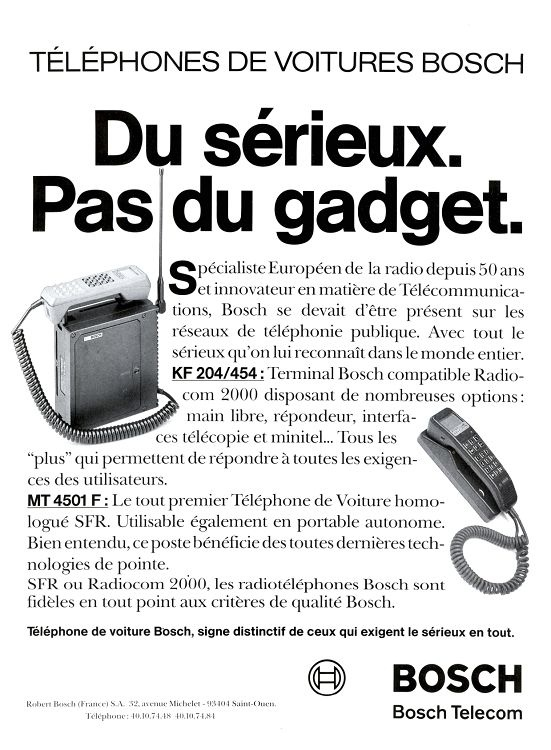
\includegraphics[width=0.70\textwidth,height=0.9\textheight]{img/bosch.jpg}
    \end{frame}

    \subsection{2G}

    \begin{frame}
        \frametitle{Global System for Mobile Communications}
        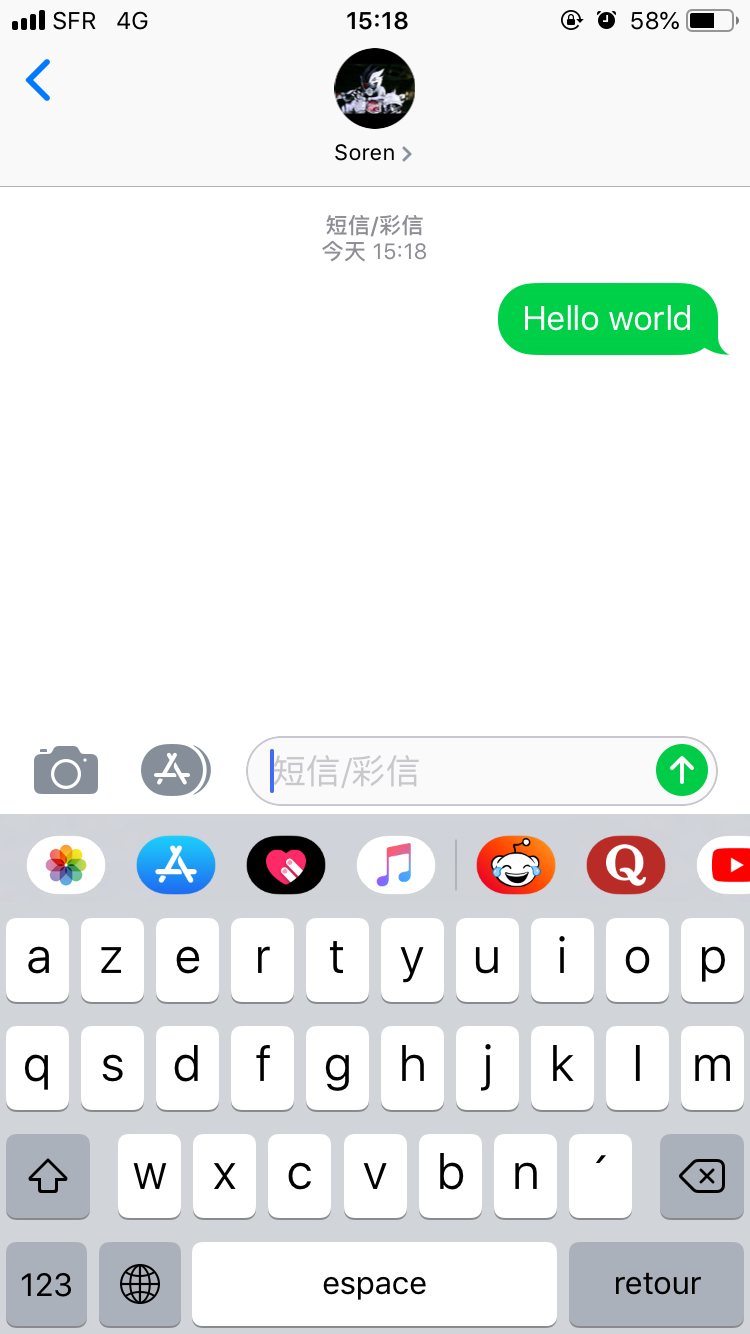
\includegraphics[width=0.5\textwidth,height=0.9\textheight]{img/sms.jpg}
        9,05 kbit/s
    \end{frame}

    \subsection{3G}
    \begin{frame}
        \frametitle{Universal Mobile Telecommunications System}
%        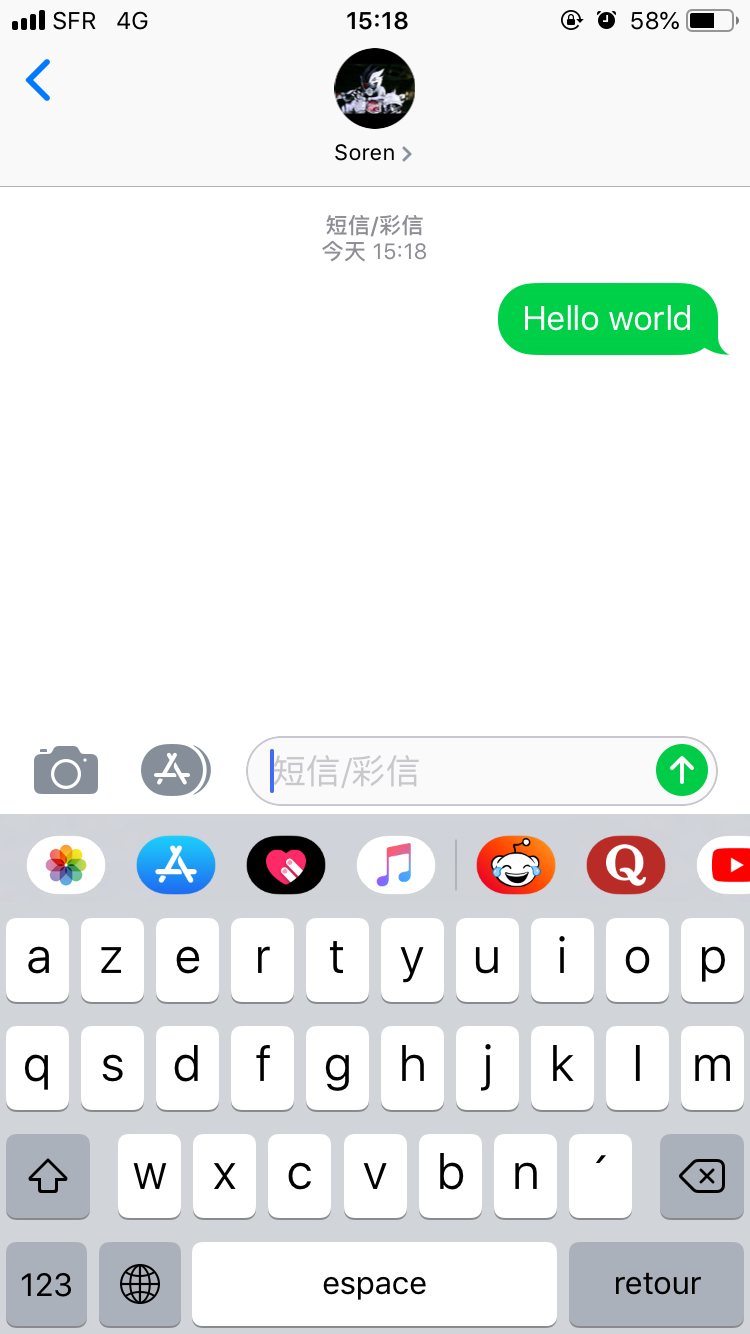
\includegraphics[width=0.5\textwidth,height=0.9\textheight]{img/sms.jpg}
        1,9 Mbit/s
    \end{frame}

    \subsection{4G}
    \begin{frame}
        \frametitle{LTE Advanced}
%        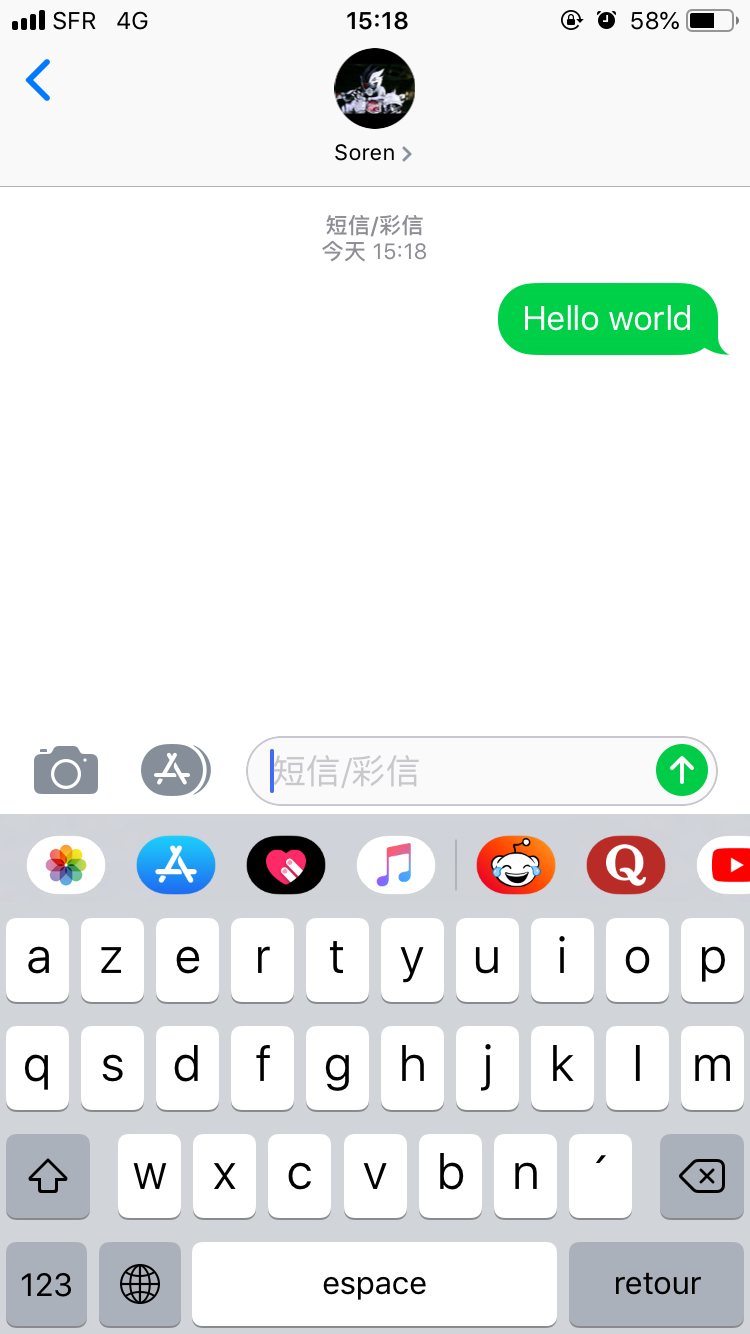
\includegraphics[width=0.5\textwidth,height=0.9\textheight]{img/sms.jpg}
        1 Gbit/s
    \end{frame}

    \section{Pourquoi la 5G}
    \begin{frame}
        \frametitle{foo}
        \begin{block}{Block name}
            Ceci est un block;
        \end{block}
        \begin{alertblock}{Block name}
            Ceci est un alertblock;
        \end{alertblock}
        \begin{exampleblock}{Block name}
            Ceci est un exampleblock;
        \end{exampleblock}

    \end{frame}
    \section{foo}
    \begin{frame}
        ehmmm
    \end{frame}
\end{document}
